\documentclass[a4paper,12pt,twoside,english,openany]{book}
\usepackage[icon=Note,color=yellow,author=Sepand]{pdfcomment}
\usepackage[utf8]{inputenc}
\usepackage[T1]{fontenc}
\usepackage{babel}
\usepackage[a4paper,left=3cm,right=2.5cm,top=3cm,bottom=3cm, twoside]{geometry}
\usepackage{xcolor}
\usepackage{stmaryrd}
\usepackage{amssymb}
\usepackage{amsmath}
\usepackage{libertine}
\usepackage[
    natbib=true,
    style=numeric,
    sorting=none
]{biblatex}

\addbibresource{res/biblio.bib} 

\usepackage[font=small,labelfont=bf]{caption}
\usepackage{subcaption}
\usepackage{float}
\usepackage{multirow}
\usepackage[Export]{adjustbox}
\usepackage{array, multirow, tabularx}
\usepackage{booktabs}
\usepackage{longtable}
\usepackage{apalike}
\usepackage{minitoc}
\usepackage{tikz}
\usetikzlibrary{calc, positioning, arrows.meta,arrows, shapes.geometric}
\usepackage[strict]{changepage}
\usepackage{siunitx}
\usepackage{enumitem}
\usepackage{epigraph}
\usepackage{lscape}
\usepackage{titletoc}
\usepackage{mdframed}
\usepackage{tabu}
\usepackage{pdfpages}
\usepackage{arydshln}
\usepackage{titling}
\usepackage{calc}
\usepackage{titlesec} 
\usepackage{sectsty}
\usepackage{lipsum}
\usepackage{emptypage}
\usepackage{fancyhdr}
\pagestyle{fancy}
\usepackage{graphicx}
\graphicspath{ {res/} }
\usepackage{hyperref} 
\hypersetup{
    colorlinks=true,
    linkcolor=black,
    filecolor=black,      
    urlcolor=black,
    citecolor=black,
    }
\definecolor{linkColor}{HTML}{32a852}

\titleformat{\chapter}[hang]
  {\normalfont\bfseries}{}{0pt}{\Huge}


%\sectionfont{\color{CentraleRed}}  % sets colour of sections
%\subsectionfont{\color{uclablue}}  % sets colour of subsections, ou gray, teal 
\definecolor{darkseagreen}{rgb}{0.56, 0.74, 0.56}

\title{Estimation of Image-Derived Arterial Input Function in Brain PET Imaging: \\ Application to Modeling PET Dynamics of Glucose Metabolism in Patients with Impaired Consciousness}
\author{Sepand Ali Madad Soltani}
\date{March 2025}



\leftmark 
\rightmark 


\usepackage[xindy]{imakeidx}
% \makeindex
%\input{auxilliaires/glossaire}
\def\mrglu{\text{MR}_{\text{glu}}}
\newcommand{\fdg}{$^{18}\text{F-FDG}$}
\begin{document}

\begin{titlepage}
	\begin{center}
		\begin{tabular}{c@{\hskip 7cm}c@{\hskip 1cm}}
			
\includegraphics[height=3cm]{res/ucbl.png} &
			
\includegraphics[height=3cm]{res/polytech.png}
		\end{tabular}
	\end{center}

	\begin{center}

		\vspace*{.03\textheight}
		\textsc{\Large University of Claude Bernard Lyon 1}\\[0.2cm]
		\large Polytech Lyon

		\rule{\textwidth}{0.8pt} \\
		\vspace{10pt}

		{\Large \bfseries \thetitle}
		\rule{\textwidth}{0.8pt} \\

	\end{center}

	\vfill
	\begin{center}
		By \textsc{\Large Sepand Ali Madad Soltani}\\[1cm]
		Master's Thesis Report\\[1.2cm]
		Supervised by \textsc{\large Inés Mérida}
		and
		\textsc{\large Nicolas Costes}  \\[0.2cm]
		Academic Advisor: \textsc{\large Kevin Tse Ve Koon}\\[0.2cm]
		November 2024 - January 2025

	\end{center}

	\vspace{1cm}
\end{titlepage}

\renewcommand{\chaptermark}[1]{\markboth{#1}{}}


\frontmatter
\chapter*{Abstract}
\lipsum[1-3]
\paragraph*{Keywords:}PET, Image-Derived, ...

\tableofcontents

\mainmatter
\setlength{\parskip}{.7em}

\renewcommand{\baselinestretch}{1.1}


\fancyhead[]{}
\fancyfoot[]{}
\fancyhead[LH]{\leftmark}
\fancyhead[RH]{\thepage}

\chapter{Introduction}
\section{Positron Emission Tomography}
Positron Emission Tomography (PET) is a functional imaging technique widely used in clinical and research settings to monitor physiological processes.
In PET, a biologically active molecule is labeled with a positron-emitting radioisotope, serving as a radiotracer, and then injected into the body.
As the radiotracer accumulates in target tissues, its radioactive decay produces positrons, which interact with electrons to emit pairs of gamma photons in nearly opposite directions.
These photons are detected by the PET scanner, and image reconstruction algorithms generate a three-dimensional representation of the tracer distribution.
This imaging modality allows for the investigation of metabolic changes, receptor binding, and other biochemical processes, providing invaluable information in oncology, neurology, cardiology, and other fields.

There are two main methods for acquiring PET images: static imaging and dynamic imaging.
Static PET involves acquiring a single scan after the radiotracer injection.
This single snapshot offers a powerful yet simplified view of tracer distribution.
The common quantification metric in static imaging is the Standardized Uptake Value (SUV), which normalizes tissue uptake by the injected dose and patient weight, allowing for a semi-quantitative comparison of tracer accumulation across different tissues or over time \cite{keyes1995suv}.
Due to its simplicity, static PET is widely used in clinical settings; however, it also has limitations.
Because it reflects only one time point, the SUV cannot capture the temporal dynamics of tracer uptake and clearance, and various physiological factors may influence its measurements, thereby reducing its accuracy.

Dynamic PET imaging provides a more comprehensive view of radiotracer kinetics by acquiring a series of images over a period ranging from a few minutes to more than an hour, depending on the tracer type.
Instead of a single snapshot, dynamic imaging produces time-activity curves (TACs) that illustrate how tracer concentration in each tissue changes throughout the scanning period.
This approach enables the measurement of physiological parameters such as the tracer rate of influx (\(K_i\)) for radiotracers with irreversible uptake (e.g. \fdg ), volume of distribution (\(V_T\)), and the rates of phosphorylation and dephosphorylation.

\section{Kinetic Modeling}
To quantify pharmacokinetic parameters, kinetic modeling is employed.
Compartmental modeling is the most popular and is considered the most accurate approach in kinetic modeling.
In compartmental modeling, the distribution and kinetics of a radiotracer are described by dividing the system into distinct compartments, each representing a pool of tracer that behaves uniformly.
Interactions between compartments can be unidirectional or bidirectional, meaning the tracer may either move in and out or only enter a compartment.
Various graphical models (e.g., the Logan \cite{logan1990graphical} and Patlak \cite{patlak1983graphical} methods), as well as classical compartmental model fitting approaches, are used to analyze tracer kinetics.

Figure~\ref{fig:2tcm} shows the irreversible two-tissue compartment model (2TCM), also known as the three-compartment model, in series mode.
This model comprises one tissue compartment for the free tracer, \(C_F(t)\), and another for the receptor-bound tracer, \(C_B(t)\), in addition to an external compartment representing the tracer concentration in the plasma or blood, denoted as the input function \(C_P(t)\).

The tracer kinetics are governed by a series of first-order differential equations, in which the exchange rates between the compartments are considered constant:
\begin{align}
	\frac{dC_F(t)}{dt} & = K_1 \, C_P(t) \;-\; \bigl(k_2 + k_3\bigr) C_F(t) \;+\; k_4 C_B(t) \,, \label{eq:2tcm-c1} \\[6pt]
	\frac{dC_B(t)}{dt} & = k_3 \, C_F(t) \;-\; k_4 \, C_B(t), \label{eq:2tcm-c2}
\end{align}
where \(K_1\), \(k_2\), \(k_3\), and \(k_4\) are the constant rate parameters.

It is generally assumed that once \fdg$ $ is phosphorylated (i.e., bound), there is little to no dephosphorylation back to the free (unbound) compartment \cite{schmidt1992errors}.
Therefore, we can set \(k_4 = 0\), treating the process as irreversible.
Thus, Equations~\eqref{eq:2tcm-c1} and \eqref{eq:2tcm-c2} simplify to
\begin{align}
	\frac{dC_F(t)}{dt} & = K_1 \, C_P(t) \;-\; \bigl(k_2 + k_3\bigr) C_F(t) \,, \\[6pt]
	\frac{dC_B(t)}{dt} & = k_3 \, C_F(t) \,.
\end{align}


\begin{figure}[b]
	\centering
	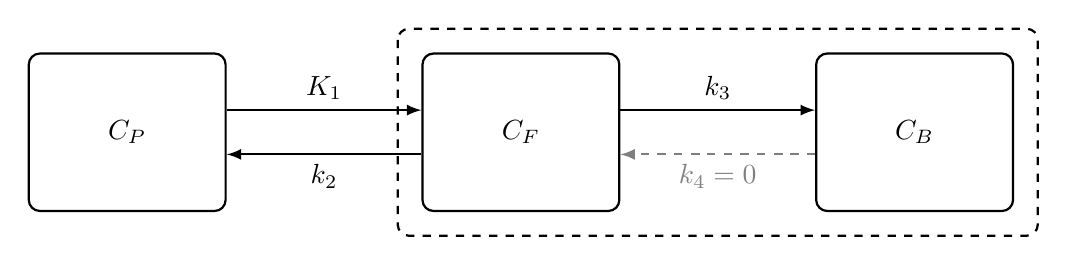
\begin{tikzpicture}[>=latex, thick]
		\node[draw, rounded corners, minimum width=2.5cm, minimum height=2cm, align=center] (Cp) at (0,0) {$C_P$};
		\node[draw, rounded corners, minimum width=2.5cm, minimum height=2cm, align=center] (C1) at (5,0) {$C_F$};
		\node[draw, rounded corners, minimum width=2.5cm, minimum height=2cm, align=center] (C2) at (10,0) {$C_B$};

		\draw[->]
		([yshift=8pt]Cp.east) to[out=0, in=180]
		node[above] {\(K_1\)}
		([yshift=8pt]C1.west);

		\draw[->]
		([yshift=-8pt]C1.west) to[out=180, in=0]
		node[below] {\(k_2\)}
		([yshift=-8pt]Cp.east);

		\draw[->]
		([yshift=8pt]C1.east) to[out=0, in=180]
		node[above] {\(k_3\)}
		([yshift=8pt]C2.west);

		\draw[->, dashed, opacity=0.5]
		([yshift=-8pt]C2.west) to[out=180, in=0]
		node[below] {\(k_4 = 0\)}
		([yshift=-8pt]C1.east);

		\draw[dashed, rounded corners, thick] ($(C1.north west)+(-0.3,0.3)$) rectangle ($(C2.south east)+(0.3,-0.3)$);

	\end{tikzpicture}
	\caption{Schematic of the irreversible two-tissue compartment model (2TCM)}
	\label{fig:2tcm}
\end{figure}

The total radiotracer tissular kinetic measured by PET (the PET data), \(C_T(t)\), is given by
\begin{equation}
	C_T(t) \;=\; C_F(t) \;+\; C_B(t) \;+\; C_P(t).
\end{equation}

Thus to solve this system of equations and to estimate \(K_1\), \(k_2\), and \(k_3\) parameters, we must fit the model using the measured PET TACs ($C_T$) and the input function ($C_P$).
% to the measured PET TACs ($C_T$), using \(C_P(t)\) as the input function.
Consequently, the influx rate (trapping rate) of \fdg$ $ in the tissue, \(K_i\), can be derived as
\begin{equation}
	K_i = \frac{K_1 \times k_3}{k_2 + k_3} \,.
\end{equation}

\fdg$ $ is an analog of glucose, not glucose itself.
To convert the \fdg$ $ trapping rate into the actual rate of glucose metabolism, both the glucose concentration and the lumped constant must be taken into account.
\begin{equation}
	\textrm{MR}_{glu} \; (\textrm{\textmu mol/min/100g}) = \frac{[C]}{LC} \cdot K_i \,.
\end{equation}
Here, \(\textrm{MR}_{glu}\) represents the metabolic rate of glucose, \([C]\) denotes the glucose concentration, and \(LC\) is the lumped constant.

\section{Input Function}
\subsection{Arterial Input Function}
The arterial input function (AIF) is considered the gold standard for obtaining the input function.
It is determined by inserting an arterial catheter into the patient and continuously drawing blood samples to measure the radiotracer concentration, thereby obtaining the blood activity curve used in the quantification model.
However, this procedure is invasive and can cause discomfort, potentially discouraging patients from undergoing future examinations.
Furthermore, this method is labor-intensive and requires trained personnel to manage both the patient and the measurement devices.

\subsection{Image Derived Input Function}
The image-derived input function (IDIF) has been proposed as a non-invasive alternative for obtaining the input function.
IDIF techniques typically involve identifying vascular structures or regions with high blood pool activity within the imaging field and extracting the input function directly from the PET images.
In brain PET imaging, the carotid arteries are the largest vessels present in the limited field of view (FOV) and have a diameter of approximately 5 mm, which is comparable to the typical spatial resolution of PET (4-6mm FWHM).
Therefore, directly extracting the carotids from PET images is impractical due to the limited resolution and the strong partial volume effects (PVE) present.

With the emergence of hybrid PET/MRI machines, it has become feasible to acquire both functional and anatomical data simultaneously.
MRI provides high-resolution soft tissue contrast, while PET captures metabolic activity.
For instance, time-of-flight MR angiography (TOF-MRA) delivers excellent arterial contrast, which allows for accurate segmentation of vascular structures such as the carotid arteries.
However, even with a high-resolution anatomical guidance, directly applying the segmented arterial mask to the PET images introduces challenges \cite{zanotti2011image}.
In particular, the limited spatial resolution of PET can lead to partial volume effects, resulting in inaccuracies in the derived input function.
Consequently, additional correction techniques are required to mitigate these effects and ensure reliable quantification.

Several methods have been developed to enhance IDIF accuracy by addressing partial volume correction and automation challenges.
Early PET-only approaches primarily focused on classical partial volume correction (PVC) techniques \cite{mourik2009image}, while more recent methods have explored supervised clustering algorithms \cite{lyoo2014image} and deep learning approaches \cite{chavan2024end,ferrante2024physically}.
Hybrid PET/MRI methods improve carotid artery delineation by leveraging anatomical imaging. The caliPER software, for instance, employs a semi-automated approach for IDIF extraction using carotid masks obtained from T1 or TOF-MRA images, incorporating partial volume correction \cite{dassanayake2022caliper}.
Additionally, fully automated methods have been proposed to enhance carotid segmentation and PVC techniques \cite{sari2017estimation, jochimsen2016fully, khalighi2018image, sundar2019towards}.

% Various techniques have been proposed for IDIF extraction in PET/MRI hybrid imaging.
% \citeauthor{dassanayake2022caliper} \cite{dassanayake2022caliper} developed caliPER; A semi-automated software for IDIF extraction using carotid masks obtained from T1 or TOF-MRA images with partial volume correction.
% Supervised clustering algorithms \cite{lyoo2014image} and deep learning pipelines \cite{chavan2024end} eliminate manual carotid segmentation.
% % \citeauthor{sundar2019towards} \cite{sundar2019towards} proposed a fully automatique technique for carotid segmentation and partial volume effect correction from TOF-MRA images.
% % Advanced in deep learning techniques gave way to techniques such as
% Recent work highlights progress in automating IDIF extraction using anatomical PET/MRI guidance and partial volume correction (PVC).
% Supervised clustering algorithms \cite{lyoo2014image} and deep learning pipelines \cite{chavan2024end} eliminate manual carotid segmentation, achieving errors <10\% compared to arterial inputs.
%
% Several methods have been developed to enhance IDIF accuracy by addressing partial volume correction and automation challenges.
% caliper; a semi-automated software for idif extraction using carotid masks obtained from t1 or tof-mra images with partial volume correction.
% It enabled blood-free quantification with minimal bias \cite{dassanayake2022caliper}.
% Supervised clustering techniques reduce noise and operator variability by automating the carotid segmentation process while maintaining accuracy \cite{lyoo2014image}.
% \citeauthor{chavan2024end} proposed an end-to-end deep learning technique to directly extract the IDIF 
% % Deep learning pipelines using 3D U-Net and RNN models further improve carotid segmentation and IDIF estimation \cite{chavan2024end}.
% Automated MR-driven IDIF extraction has shown strong agreement with arterial sampling \cite{sundar2019towards},
% % while optimized TOF-PET/MR techniques help mitigate spill-over effects in cerebral blood flow mapping \cite{khalighi2018image}.
% These advancements improve the reliability and clinical feasibility of non-invasive IDIF methods.

% Tools like caliPER \cite{dassanayake2022caliper} integrate MR-derived carotid masks with PVC for Patlak mapping, reducing bias in [18F]FDG quantification to <8\%.

% Hybrid PET/MRI protocols further validate MR-driven IDIFs, showing <5\% deviation in AUC and 3.2\% error in glucose metabolism \cite{sundar2019towards}.
% Despite advances, residual variability persists in spill-in/spill-out correction, particularly for small vessels \cite{khalighi2018image}, underscoring the need for robust, generalized PVC frameworks.

\citeauthor{irace2021bayesian} \cite{irace2021bayesian} proposed an automatique method for IDIF estimation by performing TOF-MRA driven carotid segmentation and using a Bayesian framework for incorporating prior knowledge into a geometric transfer matrix method \cite{rousset1998correction}---a classical partial volume correction technique.
In this work, the aim was to improve this method and enhance accuracy by evaluating it on a dataset of comatose patients.

\chapter{Materials and Methods}

\section{Dataset Description}
\lipsum[1-1]
\section{Carotid Segmentation}
\lipsum[1-3]
\section{IDIF Estimation}
Direct quantification with the IDIF extracted from the MRI mask of the carotids is impractical due to the strong Partial Volume Effects (PVE) in PET images. This however can be corrected by the use of the Geometric Transfer Matrix (GTM) method. This method considers the observered TAC to be the linear combination of the true real value and the other effecting regions.

\[
	\underbrace{
		\begin{bmatrix}
			C'_{carotid} \\
			C_{background}
		\end{bmatrix}
	}_{\text{Observered}}
	=
	\underbrace{
		\begin{bmatrix}
			\omega_{c \rightarrow c}  & \omega_{bg \rightarrow c}  \\
			\omega_{c \rightarrow bg} & \omega_{bg \rightarrow bg}
		\end{bmatrix}
	}_{\text{Geometric Transfer Matrix}}
	.
	\underbrace{
		\begin{bmatrix}
			C_{IF} \\
			C_{tissue}
		\end{bmatrix}
	}_{\text{Unknown}}
\]

Where $\omega_{n \rightarrow m}$ is the spill coefficient of region $n$ onto region $m$.


\section{FDG Quantification}
\lipsum[1-3]
\section{Evaluation and Assessment}
\lipsum[1-1]

\chapter{Implementation}
\lipsum

\chapter{Results}
\section{Carotid Segmentation from MRA-TOF}
The measures described in Section~\ref{sec:carotid} significantly improved carotid segmentation by effectively excluding brain lesions and undesired venous structures.
As illustrated in Figure~\ref{fig:seg_compare}, the cuboid mask plays a crucial role in this process.
Because no ground truth segmentation is available, visual inspection was used to evaluate the results, which showed that lesions and venous structures were rarely selected by the algorithm.
However, the algorithm acted overly conservative at times. It inadvertently excluded the periphery of the larger vessels or completely excluded the narrow ones.
\begin{figure}[h]
	\centering
	\begin{subfigure}{0.45\textwidth}
		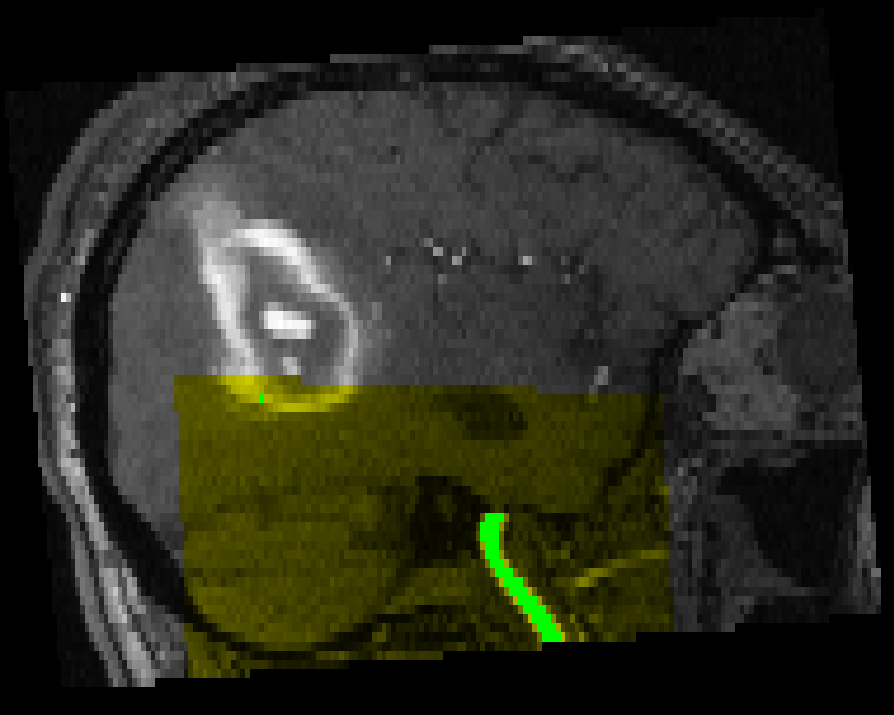
\includegraphics[width=\textwidth]{figures/molgu07704_bbox.png}
		\caption{}
		\label{subfig:seg_bbox}
	\end{subfigure}
	\begin{subfigure}{0.45\textwidth}
		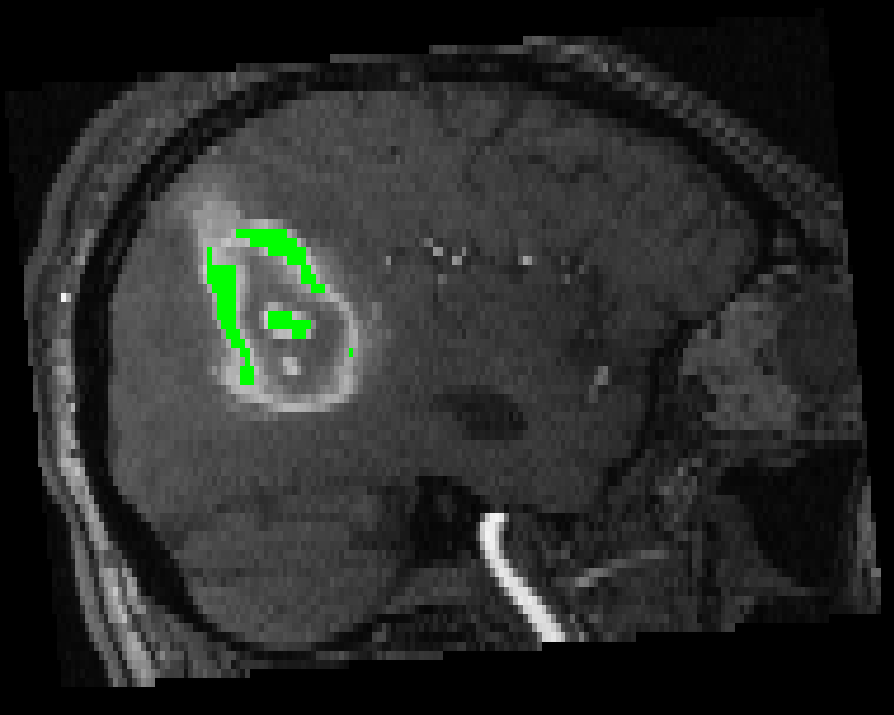
\includegraphics[width=\textwidth]{figures/molgu07704_nobbox.png}
		\caption{}
		\label{subfig:seg_nobbox}
	\end{subfigure}
	\caption{Comparison of carotid segmentation (green) with (a) and without (b) a cuboid mask (yellow). In the absence of the cuboid mask, the segmentation algorithm fails to capture the carotid and instead incorrectly identifies the brain lesion}
	\label{fig:seg_compare}
\end{figure}
\section{IDIF}
IDIF estimation was performed using both the Bayesian GTM (BGTM) and the conventional GTM PVC methods.
In Figure~\ref{fig:ifs}, we see the comparison of the two methods for one of the best and worst performing subjects.
In both cases, BGTM performed comparatively better than GTM with varying degrees.
The reason for this performance difference across subjects is not entirely clear and further analysis is needed to understand the contributing factors.
The average mean absolute error of the cAUC curves across the dataset was 14,202 for BGTM and 33,764 for GTM (Figure~\ref{subfig:cauc_boxplot}).

\begin {figure}[h]
\centering
\begin{subfigure}[b]{0.322\textwidth}
	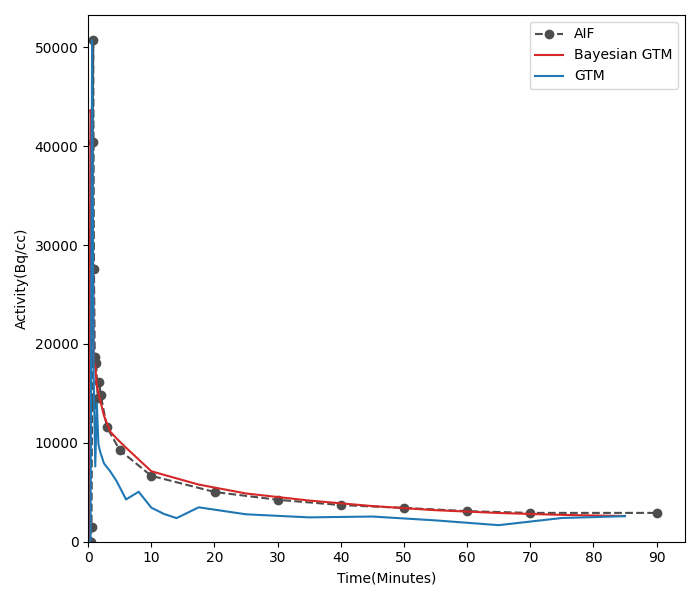
\includegraphics[width=\textwidth]{figures/MOLGU07704_1_if_comparison.png}
	\caption{}
	\label{subfig:good_if_compare}
\end{subfigure}
\begin{subfigure}[b]{0.322\textwidth}
	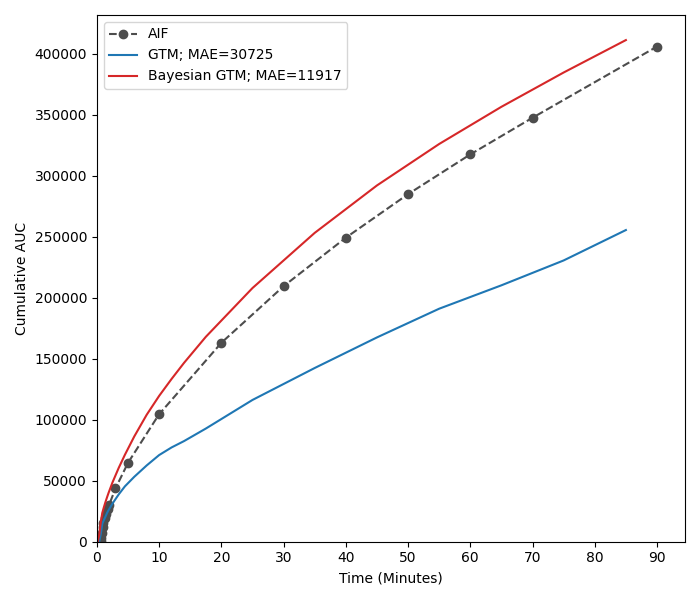
\includegraphics[width=\textwidth]{figures/MOLGU07704_1_trap.png}
	\caption{}
	\label{subfig:good_trap_compare}
\end{subfigure}
\begin{subfigure}[b]{0.322\textwidth}
	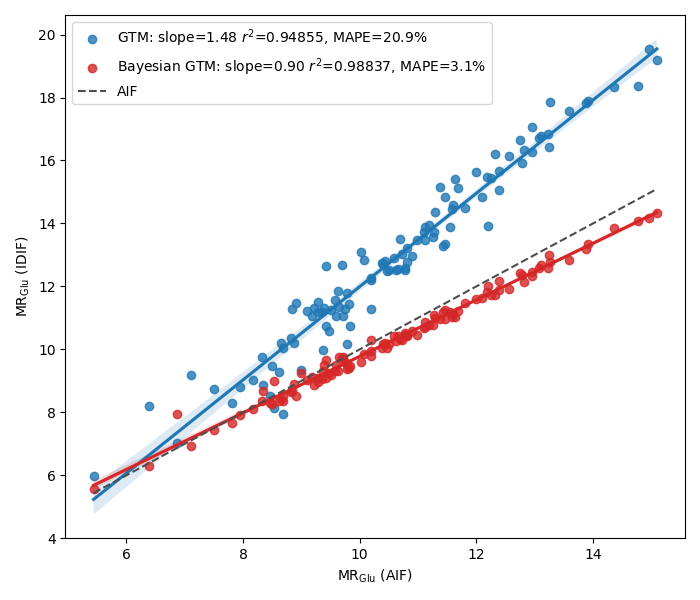
\includegraphics[width=\textwidth]{figures/MOLGU07704_1_cmrglu.png}
	\caption{}
	\label{fig:good_cmrglu}
\end{subfigure}
\begin{subfigure}[b]{0.322\textwidth}
	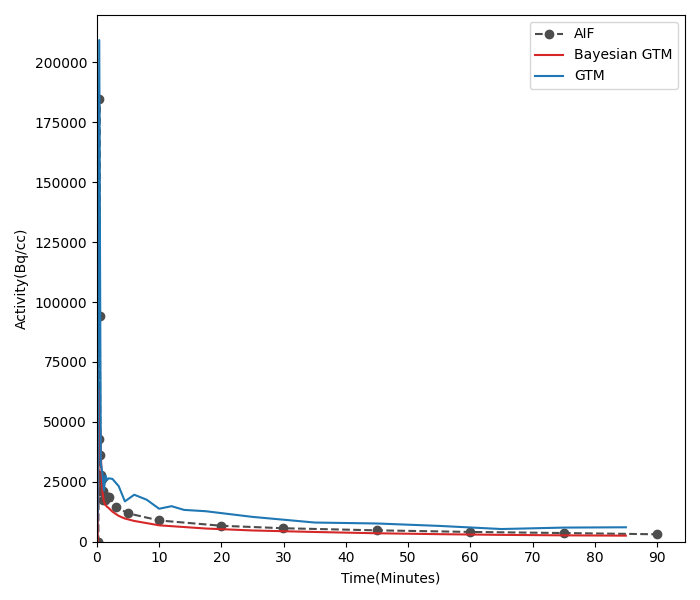
\includegraphics[width=\textwidth]{figures/SK11073_1_if_comparison.png}
	\caption{}
	\label{subfig:bad_if_compare}
\end{subfigure}
\begin{subfigure}[b]{0.322\textwidth}
	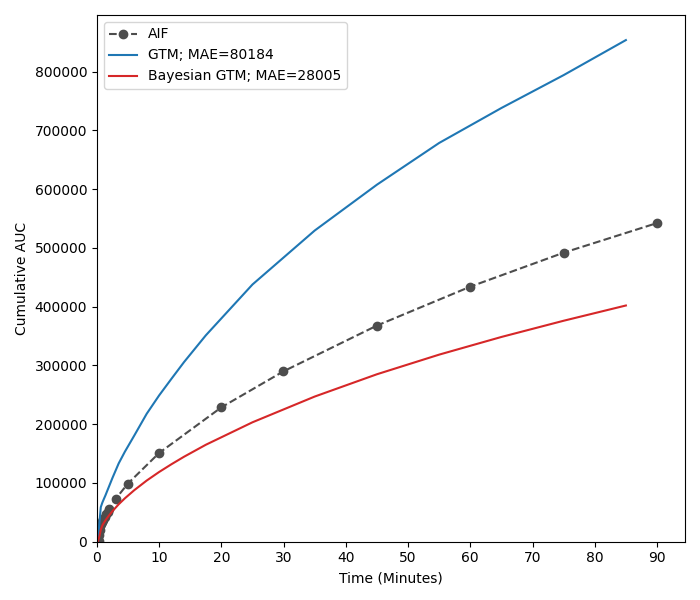
\includegraphics[width=\textwidth]{figures/SK11073_1_trap.png}
	\caption{}
	\label{subfig:bad_trap_compare}
\end{subfigure}
\begin{subfigure}[b]{0.322\textwidth}
	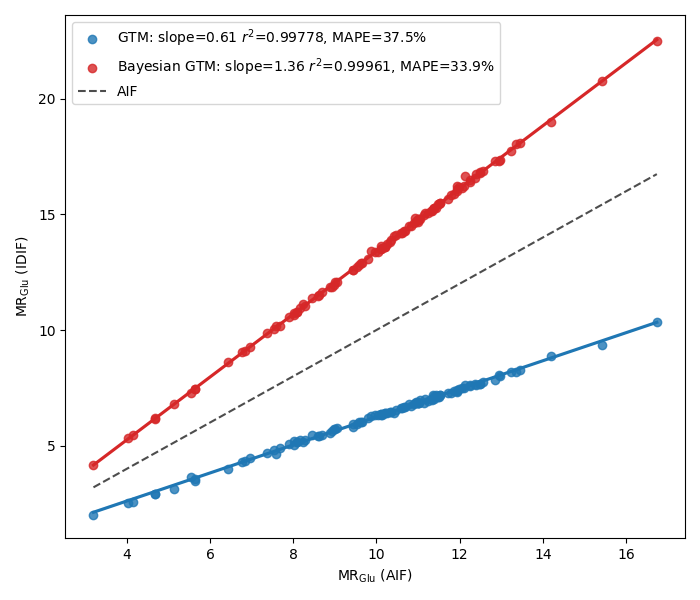
\includegraphics[width=\textwidth]{figures/SK11073_1_cmrglu.png}
	\caption{}
	\label{fig:bad_cmrglu}
\end{subfigure}
\caption{Comparison of the IFs (a,d), cumulative AUC curves (b,e), and $\mrglu$ regression lines (c,f) for one of the best (top row) and worst (bottom row) performing subjects}
\label{fig:ifs}
\end{figure}

ROI-based quantification was carried out using both IDIF methods, with BGTM yielding significantly better performance.
Specifically, the BGTM and GTM methods achieved an average \(\mrglu\) mean absolute percentage error (MAPE) of 14.1\% and 33\%, respectively (Figure~\ref{subfig:mape_boxplot}), and an average \(\mrglu\) MAE of 1.42 and 3.5.
In addition, the MAE for the coefficient of determination (\(R^2\)) and the regression slope (\(S\)) were 0.004 and 0.14 for BGTM, compared to 0.030 and 0.304 for GTM, respectively.

\begin{figure}
	\centering
	\begin{subfigure}[b]{0.45\textwidth}
		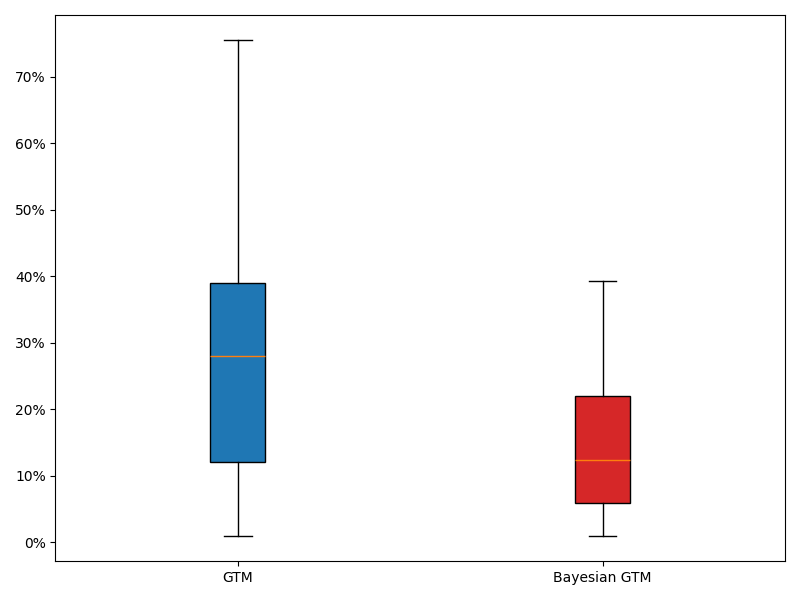
\includegraphics[width=\textwidth]{figures/quantification_mape_fitk3_boxplot.png}
		\caption{\(\mrglu\) MAPE Boxplot}
		\label{subfig:mape_boxplot}
	\end{subfigure}
	\begin{subfigure}[b]{0.45\textwidth}
		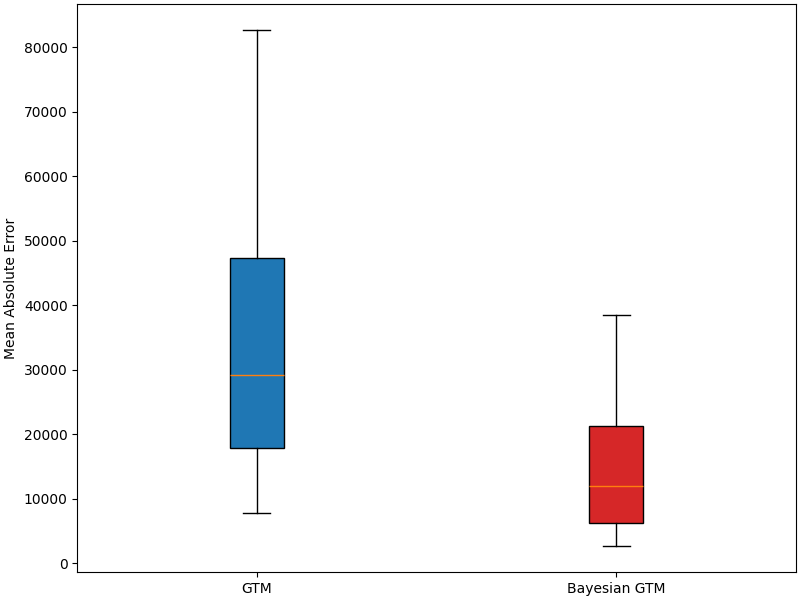
\includegraphics[width=\textwidth]{figures/curve_errors_boxplots.png}
		\caption{cAUC MAE Boxplot}
		\label{subfig:cauc_boxplot}
	\end{subfigure}
	\caption{Boxplot of curve and quantification errors}
	\label{fig:boxplots}
\end{figure}

\begin{table}[b]
	\centering
	\begin{tabular}{l|cc|cc|cc}
		\toprule
		\multirow{3}{*}{\textbf{Metric}} & \multicolumn{2}{c|}{\textbf{BGTM}} & \multicolumn{2}{c}{\textbf{GTM}} & \multicolumn{2}{c}{\textbf{Paired T-Test}}                                                 \\
		\cmidrule(lr){2-3} \cmidrule(lr){4-5} \cmidrule(lr){6-7}
		                                 & \(\mu\)                            & \(\sigma\)                       & \(\mu\)                                    & \(\sigma\) & T-Value & P-Value                \\
		\midrule
		IF cAUC MAE                      & 14,202                             & 9,190                            & 33,764                                     & 21,212     & 7.44    & \(7.2\times 10^{-10}\) \\
		$\mrglu$ MAPE (\%)               & 14.1                               & 10.1                             & 33.0                                       & 31.5       & 4.32    & \(6.5\times 10^{-5}\)  \\
		$\mrglu$ MAE                     & 1.42                               & 1.07                             & 3.50                                       & 3.38       & 4.41    & \(4.8\times 10^{-5}\)  \\
		$\mrglu$ \(R^2\) MAE             & 0.004                              & 0.006                            & 0.030                                      & 0.132      & 1.45    & \(1.5\times 10^{-1}\)  \\
		$\mrglu$ Slope MAE               & 0.14                               & 0.109                            & 0.304                                      & 0.230      & 4.73    & \(1.6\times 10^{-5}\)  \\
		\bottomrule
	\end{tabular}
	\caption{Summary of performance metrics for BGTM and GTM methods and their paired t-test.
		% $\mu$ is the average and $\sigma$ is the standard deviation
	}
	\label{tab:metrics}
\end{table}

\newpage
A paired t-test was conducted to compare the performance of BGTM and GTM across previously mentioned metrics.
The results, summarized in Table~\ref{tab:metrics}, indicate that BGTM significantly outperforms GTM in cAUC MAE(\( t = 7.44 \), \( p = 7.2 \times 10^{-10} \)), $\mrglu$ MAPE (\( t = 4.32 \), \( p = 6.5 \times 10^{-5} \)), $\mrglu$ MAE (\( t = 4.41 \), \( p = 4.8 \times 10^{-5} \)), and $\mrglu$ Slope MAE (\( t = 4.73 \), \( p = 1.6 \times 10^{-5} \)), demonstrating the effectiveness of the proposed method.
However, no significant difference was observed in $\mrglu$ \(R^2\) MAE (\( t = 1.45 \), \( p = 0.15 \)).


As illustrated in Figure~\ref{fig:corr_mat}, there is a strong correlation between the cAUC MAE and the quantification errors showing cAUC can be a good intermediate metric.

\begin{figure}[h]
	\centering
	\begin{subfigure}{0.45\textwidth}
		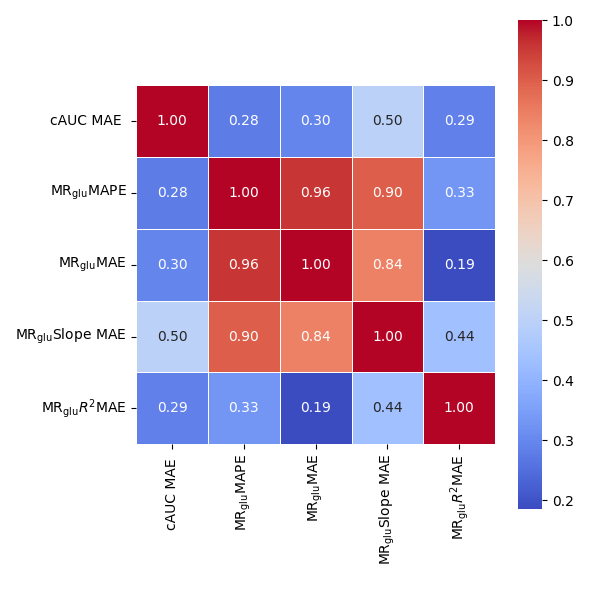
\includegraphics[width=\textwidth]{figures/corr_gtm.png}
		\caption{GTM}
		\label{subfig:corr_gtm}
	\end{subfigure}
	\begin{subfigure}{0.45\textwidth}
		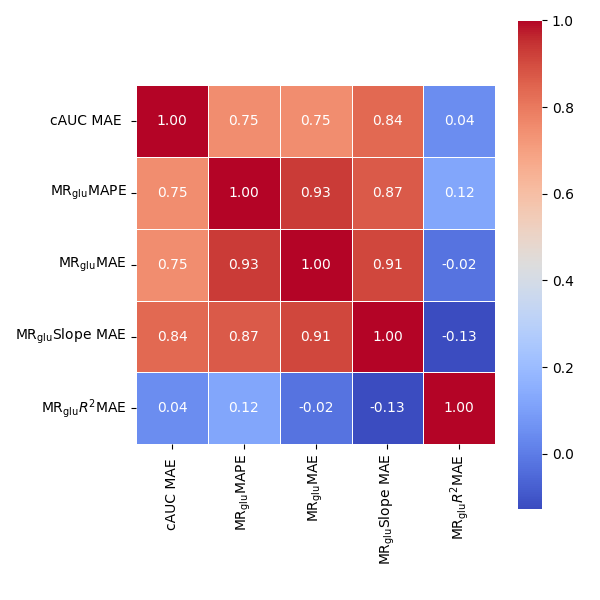
\includegraphics[width=\textwidth]{figures/corr_bgtm.png}
		\caption{Bayesian GTM}
		\label{subfig:corr_bgtm}
	\end{subfigure}
	\caption{Correlation matrix of different metrics for Bayesian GTM and GTM methods}
	\label{fig:corr_mat}
\end{figure}




\chapter{Discussion}

\lipsum

\chapter{Conclusion}
This study demonstrates that combining TOF-MRA-guided carotid segmentation with Bayesian partial volume correction improves non-invasive input function estimation for PET/MRI in comatose patients.
While the method reduces reliance on invasive sampling, residual variability underscores challenges in spill-over correction and registration accuracy between PET and MR-derived vascular masks.
Future validation must address limitations in the current PCA framework by establishing standardized reference cohorts and expanding to multi-center studies with diverse patient populations.
By refining anatomical alignment protocols and ensuring consistent prior knowledge integration, this approach can enhance reliability for clinical translation, ultimately supporting safer, patient-friendly quantitative PET imaging.

\newpage
\fancyhead{}
\fancyhead[L]{\textsc{References}}
\printbibliography[
	heading=bibintoc,
	title={References}]



\end{document}

